\subsection{Visualisierung}

\subsubsection{Aufgaben}
Die wichtigste Aufgabe sämtlicher in der Anwendung des Edubot Systems verbauten Visualisierungen ist es, den Betrieb der Software auch ohne angeschlossene Hardware zu ermöglichen. Ein wichtiger Nebenaspekt der Visualisierung ist jedoch auch die Möglichkeit zu geben, bei angeschlossener Hardware die vom Roboter getätigten Verfahrbewegungen kontrollieren zu könen.
Letztere Funktion der Visualisierung kam vor allem bei der Entwicklung der Software für die Ansteuerung des Edubot Modells, sowie bei der Entwicklung der verschiedenen Interpolationsarten sehr intensiv zum Einsatz. 

\subsubsection{Allgemeines und Aufbau}
Für die Edubot Anwendung stehen im Allgemeinen zwei Arten der Visualisierung bereit, einerseits eine Maßstabsgetreue Simmulation des Edubot Modells, andererseits eine universelle, schematische Darstellung Simulation eines Roboters mit RR Kinematik. 
Die Simulation des Edubot Modells kann in den Einstellungen nach belieben ein oder ausgeschaltet werden und kann nur mit den Achsverhältnissen des Edubot Modells betrieben werden. Für diese Simulation kann nur eine 3D Ansicht gewählt werden.
Die universelle Robotersimulation ist immer vorhanden und passt sich automatisch den eingegebenen Achslängen an. Für diese Simulation gibt es sowohl eine 3D Ansicht, als auch eine zweidimensionsale Darstellung in Form einer Ansicht von oben.

\begin{figure}[H]
  \centering
  \begin{minipage}[t]{12 cm}
  	\centering
  	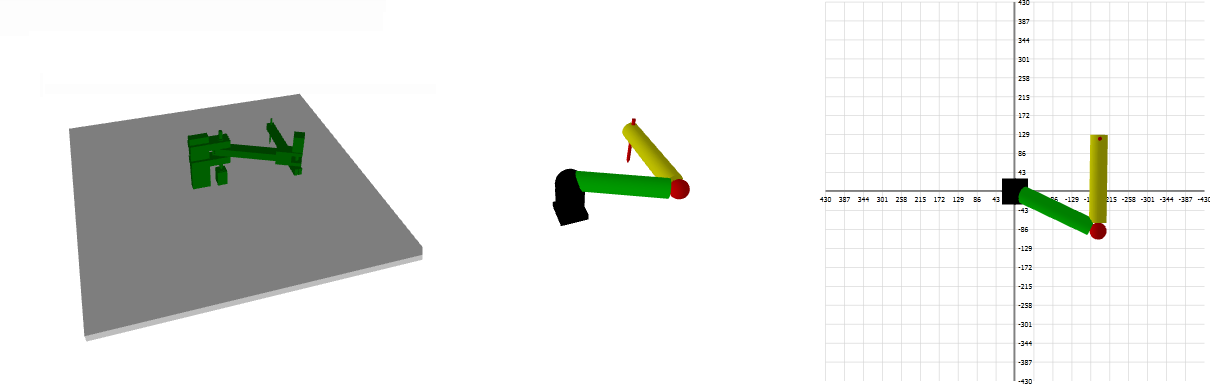
\includegraphics[width=12cm]{images/3DModels} 
    \caption{Visualisierungs-Modelle}
  \end{minipage}
\end{figure} 

Bei der Erstellung der Visualisierungen wurde jeweils zuvor ein dreidimensionales Modell in Google SketchUp angefertigt. Dieses Modell wurde durch Google SketchUp in Form einer .obj Datei exportiert und später mithilfe von Microsoft Expression Blend konvertiert. In Visual Studio wurde das Modell schließlich als UserControll implementiert und mit der nötigen Programmlogik zur Animaton versehen.
Die einzelnen Schritte werden in den nächsten Kapiteln genauer beschrieben.
\subsubsection{Anfertigung und Vorbereitung der Modelle}
Wie bereits erwähnt wurden die 3D Modelle zuerst im Programm SketchUp angefertigt. Dies ist mithilfe der von Google zur Verfügung gestellten Software bereits nach kurzer Einarbeitungszeit möglich. 
Prinzipiell basiert die Erstellung von 3D Modellen in SketchUp auf dem Prinzip, zuerst Flächen zu zeichnen und diese dann mit einem Entsprechenden Tool zu einem Körper auseinander zu "'ziehen"'.

Das fertige Modell des Roboters wurde im nächsten Schritt als "'.obj"' Datei gespeichert. Beim "'.obj"' Dateityp handelt es sich um einen von der Firma Wavefront entwickelten offenen Dateityp zur Speicherung von 3D Modellen. Das dreidimmensionsale Objekt wird dabei in seine einzelnen Formen aufgeteilt und in Form von einzelnen Koordinatennetzen die sich als normaler Text in in der Datei finden gespeichert.

Der große Vorteil der Speicherung als "'.obj"' Datei ist die vielfältige Wiederverwendbarkeit des Modells. So ist es etwa möglich, das Modell mithilfe der Software Microsoft Expression Blend zu öffnen und für die Verwendung in WPF entsprechend zu konvertieren. Die entsprechende "'.obj"' muss hierzu lediglich auf die Arbeitsfläche des XAML Designers eines WPF Projektes gezogen werden. Microsoft Expression Blend übernimmt dann alle Vorgänge die zur Umrechnung nötig sind und bettet das 3D Modell in die XAML Datei ein. 
Sämtliche Informationen zur Geometrie des Modells werden dabei in der XAML Datei gespeichert und die einzelnen Komponenten werden jeweils als \textit{GeometryModel3D} Elemente erzeugt.
Jedes dieser Elemente enthält nun in Form der Koordinatennetze eine einzelnes Objekt des 3D Modells. Um die einzelnen Objekte, bei denen es sich um um minimale Einzelteile wie beispielsweise eine Einzelne Motrwelle handelt, später nicht alle Einzeln im Programmcode ansprechen zu müssen, wurden Objekte bei der Erstellung des Modells zu Komponenten zusammengefasst. Diese Komponenten können beispielsweise eine gesamte achse mit Gelenk oder ähnliches darstellen und sind im XAML Dokument als \textit{ModelVisual3D}, welches seinerseits mehrere \textit{GeometryModel3d} Elemente enthält, definiert.
Als Übergeordnetes Element für das gesamte 3D Modell dient ein \textit{ViewPort3d} Modell dass die einzelnen Komponenten Enthält und zusätzlich über ein \textit{PerspectiveCamera} Element den Blickwinkel und verschiedene Beleuchtungsoptionen definiert.

Das eben beschriebene \textit{ViewPort3d} Überelement kann nun aus der, durch Expression Blend erstellten, XAML Datei kopiert und in eine beliebige XAML Datei in einem Visual Studio WPF Projekt eingefügt werden. Im Fall der Edubot Anwendung wurde die Visualisierung als UserControll programmiert um das einfache Einfügen an beliebigen Punkten zu ermöglichen. Aus diesem Grund wurde das \textit{Viewport3d} Objekt in XAML Datei des UserControlls eingefügt.

\subsubsection{Programmierung der Animation}
Wie im vorherigen Unterkapitel bereits erwähnt wurden die einzelnen Simulationen jeweils als UserControlls ausgegliedert und später in die Hauptanwendung integriert. 
In WPF besteht ein UserControl immer aus zwei verschidenen Dateien, einer XAML Datei als Markup des Designs und einer seperaten C\# Codedatei welche die Logik hinter dem UserControl bereitstelltl. Die XAML Datei wurde bereits im vorhergehenden Kapitel in ihren Grobzügen erklärt, wissenswert ist an dieser Stelle noch dass bei einem UserControll das Element auf der untersten Ebene ein Element vom Typ \textit{UserControll}, darüber liegt standarmäßig ein Element vom Typ \textit{Grid} welches die Anordnung der Unterlemente (in unserem Fall direkt das zuvor Erzeugte \textit{ViewlPort3D} Element) ähnlich wie bei einer Tabelle in HTML ermöglicht.

Auf die in der XAML Datei definierten Elemente kann, sofern ihnen über das \textit{name} Attribut zugewiesen wurde, aus dem Programmcode zugegriffen werden. Dieser befindet sich in der zweiten zum UserControll gehörenden Datei.

In der beschriebenen Code Datei befindet sich nun die eigentlich für die Animation benötigte Code Date. 

Für die Animation werden die in der API berrechneten Interpolationsergebnisse benötigt. Dazu besitzt der für die Visualierung verwendete Adapter einen Event (\textit{onMovementStartet}) der eine ihm zugewewiesen Methode in der Anwendung benachrichtigt wenn neue Interpolationsergebnisse zur Verfügung stehen und diese auch gleich dieser Methode übergiebt. 

In der von der API benachrichtigte Methode der Anwendung wird die Animation gestartet. Hierzu werden die \textit{Animate()} Methode des UserControlls aufgerufen und dieser die Interpolationsergebnisse übergeben.

Die \textit{Animate()} Methode startet nun einen neuen Thread um zu verhindern dass für die Zeitspanne in der die Animation läuft die Anwendung still steht. Der neue Thread führt die Methode \textit{StartAnimation()} aus, welche in einer Schleife alle im Interpolationsergebnis enthaltenen Schritte (Teilstrecken) hintereinander ausführt und die Achsen um den jeweiligen Winkel verschiebt, bzw. um die jeweilige Strecke verschiebt. 

Da es sich bei den Achsen um Objekte des ursprünglichen Threads handelt, muss für den Zugriff daruf ein Dispatcher verwendet werden. Der Zugriff mittels eines Dispatchers ermöglicht das Aufrufen einzelner Delegaten welche Methoden aufrufen die ihrerseits dann die Werte verändern, die Veränderung der Werte geschieht im urspünglichen Thread und das Dispatcher Objekt stellt eine Art Warteschlange dar. An dieser Stelle wird jedoch nicht genauer auf diesen Mechanismus eingegangen, da dies den Rahmen dieser Arbeit sprengen würde.

Das Rotieren und Verschieben der Roboterachsen kann über das WPF eigene \textit{Tranform3DGroup} Objekt, sowie über das \textit{Transform} Property der im XAML definierten \textit{ModelVisual3D} Elemente.
Hierzu wird im Code ein Objet vom Typ \textit{ Transform3DGroup} angelegt. Diesem Objekt enthält eine Liste der die durchzuführenden Transformationen angefügt werden können. Für die verschiedenen Transformationsarten stehellt WPF jeweils Klassen bereit die das Interface \textit{Transform3D} implentiert. Für unsere Animation wurden folgende Transformationsarten verwendet:

\begin{itemize}
\item \textbf{RotateTransform3D}\\
Durch ein Objekt dieser Klasse wird eine Rotation definiert. Beim Anlegen eines Objektes dieses Klasse muss ein Objekt vom Typ \textit{AxisAngleRotation3D} mitgegeben, welches speziell eine rotatorische Transformation um eine einzelne Achse definiert und über ein \textit{Vector3D} Objekt die Informationen über die Lage der Achse um die rotiert werden soll erhält. Zusätzlich müssen für das \textit{AxisAngleRotation3D} Objekt noch der zu Rotierende Winkel und optional falls nicht der Koordinatenursprung verwendet werden soll ein Mittelpunkt für die Rotation gewählt werden.

\item \textbf{ScaleTransform3D}\\
Ein Objekt der Klasse \textbf{ScaleTransform3D} defiert die Skalierung die bei seiner Anwendung auf ein Element angewendet wird. Um die Skalierung genau zu definieren muss ein Mittelpunkt (bei nicht Angabe Koordinatenursprung) mittels der Übergabe eines \textit{Point3D} Objektes definiert werden. Zusätzlich muss ein \textit{Vector3D} Objekt übergeben werden welches die eigentliche Skalierung entlang der Achsen, ausgehend vom Mittelpunkt definiert.

\item \textbf{ScaleTransform3D}\\
Durch Hinzufügen eines Objektes dieser Klasse zu einer \\textit{TransformGroup3D} wird das Element auf dass diese angewendet wird verschoben. Zur Definition wie diese Verschiebung durchgeführt werden soll wird dem \textit{TranslateTransform3D} Objekt ein \textit{Vector3D} Objekt übergeben in dem für jede Achse die Distanz um die verschoben werden soll angegeben wird.
\end{itemize}

Wurden die benötigten Transformationen in Form der beschriebenen Objekte dem \textit{ Transform3DGroup} Objekt angehängt, so kann dieses nun dem zu Transormierenden Element aus der XAML Datei übergeben werden. Dies geschieht durch einfaches Zuweisen des \textit{ Transform3DGroup} Objektes an das \textit{ Transform} Property zu Transformierenden XAML Elements. Wie erwähnt handelt es sich dabei in unserem Fall um ein Objet des Typs \textit{ModelVisual3D} durch dass jeweils eine Komponente des Modells dargestellt wird.



